\scanpage{34}
\mspage{8)}

cas contraire, distinguons deux cas.

a) $H^+=\{1\}$, donc $H=\{1,\sigma\}$, où $\sigma$ est une anti-involution.

1) Si \deleted{$\unsure{\sigma}$} $X^\sigma=\varnothing$, $\sigma$ fixe une métrique sphérique normalisée unique, OK.

2) Si $X^\sigma\ne\varnothing$ i.e. $\sigma$ une inversion, alors le choix d'une métrique sphérique comp. avec $\sigma$ revient à celui d'une paire de pts de $X$ conjugués sous $\sigma$. En particulier, le choix d'un point \inserted{$x$} de $X$ tel que $\sigma x\ne x$ définit une telle métrique sphérique.

b) $H^+\ne\{1\}$. Considérons le \inserted{unique} tore \deleted{\unsure{gr}} compact de dim $1$ $T$ qui contient $H^+$, et $T.H=N$, ext. de \deleted{$\unsure{\mathbb Z}$} $\mathbb Z/2\mathbb Z$ par $T$. Les elts \deleted{\unsure{de}} $\sigma$ de $N^-$ fixent $z,z'$, ou les intervertissent, suivant que l'élt $\ne1$ de $N/T$ opère trivialement sur $T$, ou par symétrie $t\mathrel{\unsure{\vdash\!\dashv|\mapsto}}t^{-1}$.
% slanted
\margin{\uline{C'est l'inverse !}}
Dans le premier cas l'ext. $N$ de \inserted{$\gamma=$}$\mathbb Z/2\mathbb Z$ par $T$ est triviale
\[
(H^2(\gamma,T)\simeq T^\sigma/N_\sigma(T)=T/T^2\simeq0)
\]
dans le deuxième cas on trouve
\[
H^2(\gamma,T)\simeq T^\sigma/N_\sigma(T)\simeq \underbrace{{}_2T}_{\mathbb Z/2\mathbb Z}/0\simeq\mathbb Z/2\mathbb Z,
\]

1) $N$ ext. \uline{centrale} de $\deleted{\unsure{\mathbb Z|\gamma}}\gamma$ par $T$, donc $N\simeq T\times\underset{\substack{\Vert\\\{1,\sigma\}}}{\gamma}$ ($\frac12$ direct) engendré par $T$ et un $\sigma$ \deleted{qui} anti-involutif qui \deleted{fixe $z,z'$} intervertit $z,z'$. \deleted{On voit que} \deleted{\unsure{géodésique}} celle-ci est une inversion, \deleted{\unsure{ayant|dont|qui}}

\figure{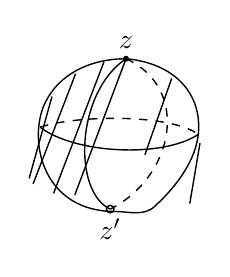
\begin{tikzpicture}[x=1cm,y=1cm,line width=.5pt]
\draw (0,.05) .. controls (-.88,.05) and (-1.1,.88) .. (-.91,1.38) .. controls (-.73,1.81) and (-.29,1.99) .. (.14,1.99) .. controls (.77,1.93) and (1.1,1.54) .. (1.06,1.05) .. controls (1.03,.70) and (.78,.37) .. (.52,.13) .. controls (.38,-.02) and (.18,.05) .. (0,.05);
\draw (.14,1.99) .. controls (-.50,1.56) and (-.54,.30) .. (-.06,.08);
\draw[dashed] (.14,1.99) .. controls (.97,1.61) and (.75,.49) .. (-.06,.08);
\draw (-.95,1.12) .. controls (-.52,.79) and (.59,.72) .. (1.06,1.03);
\draw[dashed] (-.95,1.12) .. controls (-.52,1.27) and (.68,1.30) .. (1.06,1.03);
\draw (-1.09,.47)--(-.80,1.51) (-1.04,.40)--(-.50,1.80) (-.78,.28)--(-.14,1.95) (-.51,.26)--(.14,1.99) (.38,.77)--(.72,1.74) (.95,.15)--(1.08,.92);
\fill (.14,1.99) circle (.038) node[above] {$z$}; \draw (-.06,.08) circle (.048) node[below] {$z'$};
\end{tikzpicture}}

% archive sheet number: 36
